\documentclass{article}
\usepackage{tikz}
\usetikzlibrary{positioning}

\begin{document}

\begin{figure}[h]
    \centering
    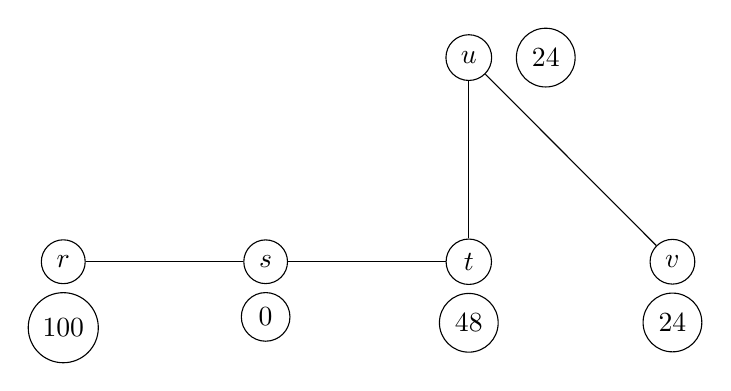
\begin{tikzpicture}[node distance=2cm, every node/.style={circle, draw, minimum size=0.5cm}]
        % Define nodes with their labels and weights
        \node (r) {$r$};
        \node[right=of r] (s) {$s$};
        \node[right=of s] (t) {$t$};
        \node[above=of t] (u) {$u$};
        \node[right=of t] (v) {$v$};

        % Draw edges between nodes
        \draw (r) -- (s);
        \draw (s) -- (t);
        \draw (t) -- (u);
        \draw (u) -- (v);

        % Add weights to the nodes
        \node[below=0.1cm of r] {100};
        \node[below=0.1cm of s] {0};
        \node[below=0.1cm of t] {48};
        \node[below=0.1cm of v] {24};
        \node[right=0.3cm of u] {24};
    \end{tikzpicture}
    \caption{The tree \( G \), weight distribution \( w \), and vertex \( v \) from the proof of~\Cref{prop:counterexample}.}
    \label{fig:counterexample}
\end{figure}

\end{document}